%%% COMPILE WITH XELATEX, NOT PDFLATEX
\documentclass[letterpaper]{article}

\usepackage[UTF8]{ctex}
\usepackage[utf8x]{inputenc}

\author{L.M Goodman}
%% \date{September 2, 2014}
\date{2014年9月2日}
%% \title{Tezos --- a self-amending crypto-ledger \\ White paper}
\title{Tezos --- 自我进化的加密账本 \\ 白皮书}
%\usepackage[utf8]{inputenc}
%%\setlength{\parskip}{\baselineskip}
\usepackage{amsfonts}
\usepackage{listings}
\usepackage{color}
\usepackage{courier}
\usepackage{epigraph}
\usepackage{fontspec}
\usepackage{newunicodechar}
\usepackage{graphicx}
\usepackage{siunitx}
\usepackage{url}
\usepackage[hidelinks]{hyperref}



%\epigraphfontsize{\small\itshape}
\setlength\epigraphwidth{4.6cm}
\setlength\epigraphrule{0pt}
%\DeclareUnicodeCharacter{42793}{\tz{}}
%Ꜩ

\usepackage{url}
\lstset{basicstyle=\footnotesize\ttfamily,breaklines=true}

\newcommand{\tz}{{\fontspec{DejaVu Sans} \small{ꜩ}}}
\begin{document}

\maketitle

%% \epigraph{\emph{``Our argument is not flatly circular,
%% but something like it.''}}
\epigraph{\emph{``我们的论点并不是简单的循环逻辑,其背后有着独到之处。''}}
{--- \textup{Willard van Orman Quine}}


\begin{abstract}
%% We present Tezos, a generic and self-amending crypto-ledger. Tezos can
%% instantiate any blockchain based ledger. The operations of a regular blockchain
%% are implemented as a purely functional module abstracted into a shell
%% responsible for network operations. Bitcoin, Ethereum, Cryptonote, etc. can all
%% be represented within Tezos by implementing the proper interface to the network
%% layer.
本白皮书向您介绍Tezos, 一个通用的且能够自我进化的加密数字账本。
Tezos的最大优势是可以吸收任何一种基于区块链的账本好的方面,其将常规区块链上的各种操作以单纯的功能模块的方式实现。
通过网络壳(Shell)利用这些操作处理网络层任务。比特币,以太坊,Cryptonote等等都可以在Tezos内通过网络层接口实现,进而被表征。

%% Most importantly, Tezos supports meta upgrades: the protocols can evolve by
%% amending their own code. To achieve this, Tezos begins with a seed protocol
%% defining a procedure for stakeholders to approve amendments to the protocol,
%% \emph{including} amendments to the voting procedure itself. This is not unlike
%% philosopher Peter Suber's Nomic\cite{Nomic}, a game built around a fully
%% introspective set of rules.

更重要的是,Tezos支持元数据升级:即可以通过自我修正代码进化协议。
为此,Tezos从一个种子协议开始定义一整套流程来让持币的用户来对代码进行修正,以及修正这套流程所必须的投票体系本身。这和哲学家Peter Suber的Nomic\cite{Nomic}博弈观点不谋而和,该观点的博弈构建主要围绕一整套内省规则。

%% In addition, Tezos's seed protocol is based on a pure proof-of-stake system
%% and supports Turing complete smart contracts. Tezos is implemented in OCaml,
%% a powerful functional programming language offering speed, an unambiguous
%% syntax and semantic, and an ecosystem making Tezos a good candidate for formal
%% proofs of correctness.
除此之外,Tezos的种子协议被放在一个纯粹的股权证明系统(POS)上,支持图灵完备的智能合约。Tezos通过OCaml 语言进行实现,该语言是一套功能强大的函数式编程语言,提供高速,非歧义语义和语法以及整个生态系统。所有的这一切让Tezos成为一个形式化正确性证明的很好的候选者。

%% Familiarity with the Bitcoin protocol and basic cryptographic primitives are
%% assumed in the rest of this paper.
以下的白皮书要求读者要对比特币协议的一定程度的了解和并理解基本的加密学知识。

\end{abstract}
\newpage

\tableofcontents
\newpage

\section{简介}
%% In the first part of this paper, we will discuss the concept of abstract
%% blockchains and the implementation of a self-amending crypto-ledger.
%% In the second part, we will describe our proposed seed protocol.

在白皮书的第一部分,我们将讨论抽象区块链的概念以及自动修正的加密账本的实现。在第二部分,我们将具体展开描述我们提出的种子协议。

\section{自动进化的加密数字账本}

一个区块链协议包含三层不同的协议:
\begin{itemize}
\item[-] 网络协议 ,发现并广播交易。
\item[-] 交易协议,定义有效交易。
\item[-] 共识协议,形成针对唯一链的共识。
\end{itemize}

%% Tezos implements a generic network shell. This shell is agnostic to the
%% transaction protocol and to the consensus protocol. We refer to the transaction
%% protocol and the consensus protocol together as a ``blockchain protocol''. We
%% will first give a mathematical representation of a blockchain protocol and then
%% describe some of the implementation choices
%% in Tezos.

Tezos实现了一个一般性的Shell。该Shell是对交易协议和共识协议是透明的。我们把交易协议和共识协议统称为区块链协议。我们将首先给区块链一个数学描述,再描述Tezos中区块链的实现选择。

\subsection{数学表达}

%% A blockchain protocol is fundamentally a monadic implementation of concurrent
%% mutations of a global state. This is achieved by defining ``blocks'' as
%% operators acting on this global state. The free monoid of blocks acting on the
%% genesis state forms a tree structure. A global, canonical, state is defined as
%% the minimal leaf for a specified ordering.
一个区块链的协议本质上是一个全局状态并发突变的单子(monadic)的实现,以区块为单位操作全局状态。区块的自由类群(free monid)从创始状态开始形成一个树状结构。一个全局标准状态就是这个树的满足一定顺序的最小叶。

%% This suggests the following abstract representation:
以下是其抽象的表达:

\begin{itemize}
\item[-] %% Let $(\mathbf{S},\leq)$ be a totally ordered, countable, set of possible
%% states.
定义$(\mathbf{S},\leq)$为一个完全排序的,可以被计数的,可能状态的子集。
\item[-]%% Let $\oslash \notin \mathbf{S}$ represent a special, invalid, state.
定义$\oslash \notin \mathbf{S}$为一个特殊的无效的状态
\item[-]%% Let $\mathbf{B} \subset \mathbf{S}^{\mathbf{S} \cup \{\oslash\}}$ be the
%% set of blocks. The set of \emph{valid} blocks is
%% $\mathbf{B} \cap \mathbf{S}^{\mathbf{S}}$.
定义$\mathbf{B} \subset \mathbf{S}^{\mathbf{S} \cup \{\oslash\}}$为区块集合。这个有效的区块集合是$\mathbf{B} \cap \mathbf{S}^{\mathbf{S}}$.
\end{itemize}

%% The total order on $\mathbf{S}$ is extended so that
%% $\forall s \in \mathbf{S}, \oslash < s$.
%% This order determines which leaf in the block tree is considered to be the
%% canonical one. Blocks in $\mathbf{B}$ are seen as operators acting on the state.
在$\mathbf{S}$之上的顺序被延续,所以这里$\forall s \in \mathbf{S}, \oslash < s$。这个顺序决定哪个叶在区块树上将被认可。$\mathbf{B}$中的区块可以看做是在这个状态上的操作。

%% All in all, any blockchain protocol\footnote{GHOST is an approach which orders
%% the leafs based on properties of the tree. Such an approach is problematic for
%% both theoretical and practical reasons. It is almost always better to emulate it
%% by inserting proofs of mining in the main chain.} (be it Bitcoin, Litecoin,
%% Peercoin, Ethereum, Cryptonote, etc) can be fully determined by the tuple:
总而言之,任何一个区块链协议\footnote{GHOST是一种可以基于树特性对叶子进行排序的方法。然而,这样的方式在理论和实践上都存在问题。与之相比,在主链添加挖矿证明几乎总是更好的解决方案。},
不论是比特币,莱特币,点点币,以太坊,还是Cryptonote,等等,都可以用以下元组来决定:
%% $$\left(\mathbf{S},\leq,\oslash,
%% \mathbf{B} \subset \mathbf{S}^{\mathbf{S} \cup \{\oslash\}}\right)$$
$$\left(\mathbf{S},\leq,\oslash,
\mathbf{B} \subset \mathbf{S}^{\mathbf{S} \cup \{\oslash\}}\right)$$

%% The networking protocol is fundamentally identical for these blockchains.
%% ``Mining'' algorithms are but an emergent property of the network,
%% given the incentives for block creation.
这些区块链的网络层协议基本相同。其挖矿算法却发展迅速,激励着区块的创建。

%% In Tezos, we make a blockchain protocol introspective
%% by letting blocks act on the protocol itself.
%% We can then express the set of protocols recursively as
%% $$\mathcal{P} = \left\{\left(\mathbf{S},\leq,\oslash,\mathbf{B} \subset
%% \mathbf{S}^{(\mathbf{S} \times \mathcal{P})\cup \{\oslash\}} \right)\right\}$$
在Tezos中,我们设计能够自省的区块链协议,让区块在协议层上运作。这样我们就能够递归地表示这组协议:
$$\mathcal{P} = \left\{\left(\mathbf{S},\leq,\oslash,\mathbf{B} \subset
\mathbf{S}^{(\mathbf{S} \times \mathcal{P})\cup \{\oslash\}} \right)\right\}$$

\subsection{网络Shell}
%% This formal mathematical description doesn't tell us \emph{how} to build the
%% block tree. This is the role of the network shell, which acts as an interface
%% between a gossip network and the protocol.
仅有一个形式的数学表述并不足以让我们立刻建立一个区块树。我们还需要一个连接Gossip网络和协议的网络Shell。

%% The network shell works by maintaining the best chain known to the client. It is
%% aware of three type of objects. The first two are transactions and blocks, which
%% are only propagated through the network if deemed valid. The third are
%% protocols, OCaml modules used to amend the existing protocol. They will be
%% described in more details later on. For now we will focus on transaction and
%% blocks.
这个网络Shell通过维护客户端所知的最优链进而运作。它将从三种对象那里接受信息。前两个分别是交易和区块,确认有效后广播。第三个是协议,即用来修改现有协议的OCaml模块,对此我们稍后再进行详细描述。
现在我们主要关注交易和区块。

%% The most arduous part of the network shell is to protect nodes against
%% denial-of-service attacks.
网络Shell最艰巨的部分是保护节点免于遭受DOS攻击。

\subsubsection{时钟}
%% Every block carries a timestamp visible to the network shell. Blocks that appear
%% to come from the future are buffered if their timestamps are within a few
%% minutes of the system time and rejected otherwise. The protocol design must
%% tolerate reasonable clock drifts in the clients and must assume that timestamps
%% can be falsified.
每个区块都有时间戳,这个时间戳只对网络外壳可视。如果一个区块是当前的,并且其时间戳在系统时间的几分钟之内,则该区块会被缓冲,否则将会被拒绝。这个协议设计必须能够容忍合理的时钟漂移,而且必须假设时间戳可能会被伪造。

\subsubsection{链选择算法}
%% The shell maintains a single chain rather than a full tree of blocks. This chain
%% is only overwritten if the client becomes aware of a strictly better chain.
该Shell维护一条单一的链,而不是一个完整的区块树。这个链只有在客户端获悉严格意义上的更优链时才会被覆盖。

%% Maintaining a tree would be more parsimonious in terms of network communications
%% but would be susceptible to denial-of-service attacks where an attacker produces
%% a large number of low-scoring but valid forks.
从网络通信的角度,维护一个区块树会更加节省资源,但也会让网络更加容易被DDOS攻击,尤其是当一个攻击者产生大量的低得分但有效分叉的时候。

%% Yet, it remains possible for a node to lie about the score of a given
%% chain, a lie that the client may only uncover after having processed a
%% potentially large number of blocks. However, such a node can be subsequently
%% ignored.
但仍然存在一种可能,一个节点谎报了链的得分,客户端可能会在处理大量的区块,发现和揭露该信息谎报,。随后这个欺骗节点将被忽略。

%% Fortunately, a protocol can have the property that low scoring chains exhibit a
%% low rate of block creation. Thus, the client would only consider a few blocks of
%% a ``weak'' fork before concluding that the announced score was a lie.
幸运的是,对于协议而言,低得分的链创建区块的等级越低。因此,客户端可能只需要查看一个弱分叉的几个区块,就可以判断它是不是某链的得分是不是欺骗。

\subsubsection{网络层防御}
%% In addition, the shell is ``defensive''.
%% It attempts to connect to many peers across various IP ranges. It detects
%% disconnected peers and bans malicious nodes.
此外,Shell还具备防御性。它尝试连接不同IP端的对等节点,发现掉线的节点以及禁止恶意节点。

%% To protect against certain denial of service attacks, the protocol provides the
%% shell with context dependent bounds on the size of blocks and transactions.
为防御某些DOS攻击,协议可提供Shell依赖区块大小和交易限制的环境。
\subsection{功能表述}

\subsubsection{验证链}

%% We can efficiently capture almost all the genericity
%% of our abstract blockchain structure with the following OCaml types.
%% To begin with, a block header is defined as:
我们可以通过以下的OCaml类型有效捕捉几乎所有的抽象区块链结构的继承类。从定义区块头开始:
\lstset{
  language=[Objective]Caml
}
\begin{lstlisting}
type raw_block_header = {
  pred: Block_hash.t;
  header: Bytes.t;
  operations: Operation_hash.t list;
  timestamp: float;
}
\end{lstlisting}

%% We are purposefully not typing the header field more strongly so it can
%% represent arbitrary content. However, we do type the fields necessary for the
%% operation of the shell. These include the hash of the preceding block, a list of
%% operation hashes and a timestamp. In practice, the operations included in a
%% block are transmitted along with the blocks at the network level. Operations
%% themselves are represented as arbitrary blobs.
我们故意没有把区块头域强制类型化,以致于其能够表征任意内容。但我们有必要明确类型化Shell的相关操作。这些包括前区块的哈希,一个操作哈希的列表以及时间戳。在实践中,包含在一个区块内部的操作和区块一起在网络层上传播。
操作本身可表征为任意的blobs结构.

\begin{lstlisting}
type raw_operation = Bytes.t
\end{lstlisting}

%% The state is represented with the help of a \textbf{Context} module which
%% encapsulates a disk-based immutable key-value store. The structure of a
%% key-value store is versatile and allows us to efficiently represent a wide
%% variety of states.
\textbf{Context}模块封装了一个基于磁盘的不可变化的键值对存储,在其帮助下表征状态。键值对结构十分通用,允许我们有效且广泛表征许多种状态。

\begin{lstlisting}
module Context = sig
   type t
   type key = string list

   val get: t -> key -> Bytes.t option Lwt.t
   val set: t -> key -> Bytes.t -> t Lwt.t
   val del: t -> key -> t Lwt.t
   (*...*)
end
\end{lstlisting}

%% To avoid blocking on disk operations, the functions use the asynchronous monad
%% Lwt\cite{LWT}. Note that the operations on the context are purely functional:
%% \textbf{get} uses the \textbf{option} monad rather than throwing an exception
%% while \textbf{set} and \textbf{del} both return a new \textbf{Context}.
%% The \textbf{Context} module uses a combination of memory caching and disk
%% storage to efficiently provide the appearance of an immutable store.
为避免磁盘操作的阻塞,函数使用异步单子Lwt\cite{LWT}。注意,这个操作在上下文中是纯函数式的:
当\textbf{set}和\textbf{del}都返回一个新\textbf{Context}对象时,\textbf{get}操作使用\textbf{option}单子而非抛出异常。
\textbf{Context}对象模块将内存缓存和磁盘存储结合有效提供不可变化的存储环境。

%% We can now define the module type of an arbitrary blockchain protocol:
现在我们能够定义任意区块链协议的模块类型:

\begin{lstlisting}
type score = Bytes.t list
module type PROTOCOL = sig
   type operation
   val parse_block_header : raw_block_header -> block_header option
   val parse_operation :  Bytes.t -> operation option

   val apply :
     Context.t ->
     block_header option ->
     (Operation_hash.t * operation) list ->
     Context.t option Lwt.t

   val score : Context.t -> score Lwt.t
   (*...*)
end
\end{lstlisting}

%% We no longer compare states directly as in the mathematical model, instead we
%% project the \textbf{Context} onto a list of bytes using the \textbf{score}
%% function. List of bytes are ordered first by length, then by
%% lexicographic order. This is a fairly generic structure, similar to the one used
%% in software versioning, which is quite versatile in representing various
%% orderings.
不是和数学模型做状态比对,相反,我们利用\textbf{score}函数将\textbf{Context}对象映射到一个字节列表。字节列表首先按长度排列,其次依照字母顺序。类似于软件的版本化,这是一个相当通用的结构,在表示不同排序时有着广泛应用。

%% Why not define a comparison function within the protocol modules? First off it
%% would be hard to enforce the requirement that such a function represent a
%% \emph{total} order. The score projection always verifies this (ties can be
%% broken based on the hash of the last block). Second, in principle we need
%% the ability to compare states across distinct protocols. Specific protocol
%% amendment rules are likely to make this extremely unlikely to ever happen,
%% but the network shell does not know that.
为什么不在协议模块中定义比较函数?
首先表征一个完全排序函数的需求很难执行。这经常可以从得分映射上得到验证(在上一个区块哈希的基础上破坏连接)。
其次,原则上我们需要有对比不同协议状态的能力。具体的协议修改规则可能让这个发生的可能性变得非常低,但是网络Shell对此并不知晓。

%% The operations \textbf{parse\_block\_header} and \textbf{parse\_operation} are
%% exposed to the  shell and allow it to pass fully typed operations and blocks to
%% the protocol but also to check whether these operations and blocks are
%% well-formed, before deciding to relay operations or to add blocks to the local
%% block tree database.
在决定中继操作或者添加区块至本地区块树状数据库之前,\textbf{parse\_block\_header}和\textbf{parse\_operation}操作将暴露给网络Shell,并允许其将完全类型化的操作和区块送至协议层,还要检测这些操作和区块是否经过严格封装。

%% The apply function is the heart of the protocol:
协议的核心是apply函数:

\begin{itemize}
\item[-] %% When it is passed a block header and the associated list of operations,
%% it computes the changes made to the context and returns a modified copy.
%% Internally, only the difference is stored, as in a versioning system,
%% using the block's hash as a version handle.
当传一个区块头部以及附属的操作列表时,它会计算上下文中做出的变化,返回一个修改过的副本。在内部,只有变化才会保存,和版本系统中一样,类似版本处理一样使用区块的哈希。
\item[-] %%When it is only passed a list of operations, it greedily attempts
%% to apply as many operations as possible. This function is not necessary for the
%% protocol itself but is of great use to miners attempting to form valid blocks.
当只是传操作列表时,它将贪心地试图尽可能生效更多的操作。对于协议自身而言该函数不是必须的,但对于试图形成有效区块的矿工来说却有极大的用处。
\end{itemize}

\subsubsection{协议进化}

%% Tezos's most powerful feature is its ability to implement protocol capable
%% of self-amendment. This is achieved by exposing two procedures functions to the
%% protocol:
Tezos最强大的特性是它的协议自我修正能力,主要通过暴露给协议两个过程函数实现:

\begin{itemize}
\item[-] %% \textbf{set\_test\_protocol} which replaces the protocol
%% used in the testnet with a new protocol (typically one that has been adopted
%% through a stakeholder voter).
\textbf{set\_test\_protocol}函数,使用新协议替代测试网络中使用的协议 (通常是持币者投票决定的协议)。
\item[-] %% \textbf{promote\_test\_protocol} which replaces the current
%% protocol with the protocol currently being tested
\textbf{promote\_test\_protocol}函数,用当前通过测试的协议替代目前正在运行的协议。
\end{itemize}

%% These functions transform a Context by changing the associated protocol.
%% The new protocol takes effect when the following block is applied to the chain.
这些函数通过改变目前相关联的协议来转换Context对象。当下一个区块在链上产生,新的协议开始生效。

\begin{lstlisting}
module Context = sig
   type t
   (*...*)
   val set_test_protocol: t -> Protocol_hash.t Lwt.t
   val promote_test_protocol: t -> Protocol_hash.t -> t Lwt.t
end
\end{lstlisting}

%% The \textbf{protocol\_hash} is the \textbf{sha256} hash of a tarball of
%% \textbf{.ml} and \textbf{.mli} files. These files are compiled on the
%% fly. They have access to a small standard library but are sandboxed
%% and may not make any system call.
\textbf{protocol\_hash}函数是\textbf{.ml}和\textbf{.mli}文件sha256哈希的tarball打包。这些文件在运行中编译,有获取较少的标准函数库权限,但被装在沙箱内,可能无法调用系统函数。

%% These functions are called through the \textbf{apply} function of the protocol
%% which returns the new \textbf{Context}.
这些函数通过协议的\textbf{apply}函数调用,返回新的\textbf{Context}对象。

%% Many conditions can trigger a change of protocol. In its simplest version,
%% a stakeholder vote triggers a change of protocol. More complicated rules
%% can be progressively voted in. For instance, if the stakeholder desire they
%% may pass an amendment that will require further amendments to provide a
%% computer checkable proof that the new amendment respects certain properties.
%% This is effectively and algorithmic check of ``constitutionality''.
很多条件可能会触发协议的修改。在最初的简单版本上,持币者可以通过直接投票进行协议修改, 而之后更复杂的协议可以通过逐步投票而获得接受。
例如,当一个持币者希望一个修改案被通过,他会被要求提供计算机可以验证的证据来证明他的提案将会尊重协议的某些特性。这是对协议修改合规性在算法上的有效检测。

\subsubsection{RPC}
%% In order to make the GUI building job's easier, the protocol exposes a JSON-RPC
%% API. The API itself is described by a json schema indicating the types of the
%% various procedures. Typically, functions such as \textbf{get\_balance} can
%% be implemented in the RPC.
为了简易化图形化工作,这个协议暴露了JSONRPC的API。该API自身可以被描述为一个代表各种过程类型的json模式。通常涞说,诸如\textbf{get\_balance}的函数都可以通过RPC来实现。

\begin{lstlisting}
type service = {
  name : string list ;
  input : json_schema option ;
  output : json_schema option ;
  implementation : Context.t -> json -> json option Lwt.t
}
\end{lstlisting}

%% The name is a list of string to allow namespaces in the procedures. Input and
%% output are optionally described by a json schema.
这个名字是一个字符串列表,其目的是允许过程中出现命名空间。输入和输出是通过可选择性使用json 模式刻画。

%% Note that the call is made on a given context which is typically a recent ancestor
%% of the highest scoring leaf. For instance, querying the context six blocks above
%% the highest scoring leaf displays the state of the ledger with six confirmations.
注意这个指令被用来在一个指定的上下文中,而这个上下文通常是最高得分叶子节点的最近一个祖先。
例如,在最高得分叶子节点之上查询上下文6个区块,将会显示具有六个确认的账本状态。

%% The UI itself can be tailored to a specific version of the protocol, or generically
%% derived from the JSON specification.
界面本身可以裁剪至特定的协议版本,或者是由JSON数据继承而来。

\section{种子协议}
Much like blockchains start from a genesis hash, Tezos starts with a seed
protocol. This protocol can be amended to reflect virtually any blockchain based
algorithm.
更像是区块链开始于一个创世哈希,Tezos开始于一个种子协议。这个协议可以被修改来反映几乎任何一个基于区块链的算法。

\subsection{经济}

\subsubsection{币量}
%% There are initially $\num{10000000000}$ (ten billion) coins, divisible up to two
%% decimal places. We suggest that a single coin be referred to as a ``tez''
%% and that the smallest unit simply as a cent. We also suggest to use the
%% symbol \tz~(\verb!\ua729!, ``Latin small letter tz'') to represent a tez.
%% Therefore 1 cent = \tz\num{0.01} = one hundreth of a tez.
Tezos一开始就会有一百亿个币,这些币小数点后保留两位。一个币被称作1tez,而最小的单位是分。
我们也建议使用\tz~(\verb!\ua729!, ``Latin small letter tz'') 拉丁字母来代表一个tez。这样的话,一分等于0.01tez,等于百分之一tez。

\subsubsection{挖矿和签名奖励}

\paragraph{原则}
%% We conjecture that the security of any decentralised currency requires
%% to incentivize the participants with a pecuniary reward. As explained in the
%% position paper, relying on transaction costs alone suffers from a tragedy of the
%% commons. In Tezos, we rely on the combination of a bond and a reward.
我们认为任何一个去中心化的货币要保证安全性都需要给予参与者金钱上的奖励。
正如在我们的定位白皮书中提到的,仅仅依赖于交易费进行激励会受到公共地悲剧影响。
在Tezos中,我们提供一个债券和现金奖励的二元激励体系。

%% Bonds are one year security deposits purchased by miners.
%% In the event of a double signing, these bonds are forfeited.
债券是矿工所购买的一年期的安全存款。当出现双重签名的情况下,这些债券将会被收回。

%% After a year, the miners  receive a reward along with their bond to compensate
%% for their opportunity cost. The security is primarily being provided by the
%% value of the bond and the reward need only be a small percentage of that value.
一年以后,矿工除了债券以外还将获得另外的奖励,作为他们机会成本的补偿。
债券和奖励的价值是系统安全的最主要保证,而它们的价值将仅占全部价值的一小部分。

%% The purpose of the bonds is to diminish the amount of reward needed, and perhaps
%% to use the loss aversion effect to the network's advantage.
债券的真正目的是减少奖励的总量,并利用人对损失的普遍抗拒心理来提高网络的安全。

\paragraph{细则}
%% In the seed protocol, mining a block offers a reward of \tz\num{512} and
%% requires a bond of \tz\num{1536}. Signing a block offers a reward of
%% $32\Delta T^{-1}$ tez where $\Delta T$ is the time interval in minutes between
%% the block being signed and its predecessor. There are up to 16 signatures per block
%% and signing requires no bond.
根据种子协议,每挖一个块将获得512Tezos币现金奖励以及需要1536币的债券。而每个区块签名将获得$32\Delta T^{-1}$个tez的奖励。
这里$\Delta T$代表以分钟为单位的区块和先前区块之间签名的时间间隔。每个区块至多有16个签名,但签名不需要持有债券。

%% Thus, assuming a mining rate of one block per minute, about 8\% of the initial
%% money mass should be held in the form of safety bonds after the first year.
假设出块率为每分钟一个区块,那么有8\%的最初货币供应量在第一年后应该以安全债券的形式被持有。

%% The reward schedule implies at most a 5.4\% \emph{nominal} inflation
%% rate. \emph{Nominal} inflation is neutral, it neither enrishes nor
%% impoverishes anyone\footnote{In contrast, Bitcoin's mining inflation impoverishes
%% Bitcoin holders as a whole, and central banking enrishes the financial
%% sector at the expense of savers}.
我们的奖励的计划被设定为5.4\%的通货膨胀率。这个名义上的通货膨胀应该是中性的,它不会让有的人变富,而让其他人变穷。
\footnote{与之相比, 比特币的挖矿的通货膨胀让比特币的持有者整体变穷,而中央银行又让金融界变得有钱,而让储户变穷。}.

%% Note that the period of a year is determined from the block's timestamps, not
%% from the number of blocks. This is to remove uncertainty as to the length of
%% the commitment made by miners.
请注意这里的一年周期是根据区块的时间戳而不是区块的数量决定的,这是为了抵消矿工挖矿算力不同导致的不确定性。

\paragraph{展望}
%% The proposed reward gives miners a 33\% return on their bond.
%% This return needs to be high in the early days as miners and signers commit
%% to hold a potentially volatile asset for an entire year.
这个奖励机制将给矿工33\%的债券回报。这个回报在初期必须要足够高,因为矿工和签名者需要共同持有一整年易波动的债券资产。

%% However, as Tezos mature, this return could be gradually lowered to the
%% prevailing interest rate. A nominal rate of inflation below 1\% could safely be
%% achieved, though it's not clear there would be any point in doing so.
但是,随着Tezos的成熟,这个回报可以被逐渐降低到一个同期的主流利率水平,并长期维持低于1\%的形式通胀率,但是这样做的合理性还需要进一步论证。

\subsubsection{丢失的币}
%% In order to reduce uncertainty regarding the monetary mass, addresses
%% showing no activity for over a year (as determined by timestamps)
%% are destroyed along with the coins they contain.
为了减少货币基数变化所带来的不确定性,所有的没有任何动作的地址和地址上所包含的币超过一年(由时间戳决定)都会被销毁。

\subsubsection{修改规则}
%% Amendments are adopted over election cycles lasting $N = 2^{17} = \num{131072}$
%% blocks each. Given the  a one minute block interval, this is about three
%% calendar months. The election cycle is itself divided in four quarters of
%% $2^{15} = \num{32768}$ blocks. This cycle is relatively short to encourage early
%% improvements, but it is expected that further amendments will increase the
%% length of the cycle. Adoption requires a certain quorum to be met. This quorum
%% starts at $Q = 80\%$ but dynamically adapts to reflect the average
%% participation. This is necessary if only to deal with lost coins.
 协议修改的生效时间取决于选举周期,每个周期的长度为$N = 2^{17} = \num{131072}$个区块时间。
 考虑到区块间隔是一分钟,所以这个间隔是三个月。这个选举的周期将$2^{15} = \num{32768}$个区块分成四阶段。
这个周期相对比较短,这主要是为了激励早期的协议的改善。随着未来的修改,这个周期最终将变长。
选举结果的生效需要满足一定的法定人数。法定人数开始于$Q = 80\%$,但会为了反映平均参与度而动态适应。当且仅当需要处理丢失的币时,这些才是必须的。

\paragraph{第一阶段}
%% Protocol amendments are suggested by submitting the hash of a tarball of
%% \verb!.ml! and \verb!.mli! files representing a new protocol. Stakeholders may
%% approve of any number of these protocols. This is known as ``approval voting'',
%% a particularly robust voting procedure.
建议修改协议需要提交一个代表新协议的\verb!.ml!和\verb!.mli!文件的tarball打包的哈希。持币人可能会批准任意数量的所提交协议。这也就是批准投票,是一个强健的投票过程。

\paragraph{第二阶段}
%% The amendment receiving the most approval in the first quarter is now subject to
%% a vote. Stakeholders may cast a vote for, against or can choose to explicitely
%% abstain. Abstentions count towards the quorum.
在第一阶段获得最多批准的修改案基础上进行投票。投票人可以投票反对或者弃权。投弃权的人也按法定人数计算。

\paragraph{第三阶段} %% If the quorum is met (including explicit abstentions),
%% and the amendment received $80\%$ of yays, the amendment is approved and
%% replaces the test protocol. Otherwise, it is rejected.
%% Assuming the quorum reached was $q$, the minimum quorum $Q$ is updated as such:
%% $$Q \leftarrow 0.8 Q + 0.2 q.$$
如果达到法定人数(包括明确的弃权),并且修改案达到了$80\%$的支持率, 那么修改案就会被批准,并替代测试协议。否则它将被否决。
假设法定人数达到值为$q$,按如下方式更新最小法定人数$Q$ :
$$Q \leftarrow 0.8 Q + 0.2 q.$$

%% The goal of this update is to avoid lost coins causing the voting procedure to
%% become stuck over time. The minimum quorum is an exponential moving average of
%% the quorum reached over each previous election.
做出以上更新是为了避免因为丢失币的问题延缓投票过程。最小法定人数是达到前面选举法定人数以上的指数滑动平均。

\paragraph{第四阶段} %% Assuming the amendment was approved, it will have
%% been running in the testnet since the beginning of the third quarter.
%% The stakeholders vote a second time to confirm they wish to promote the test
%% protocol to the main protocol. This also requires the quorum to be met and an
%% $80\%$ supermajority.
假定修改案被批准,在第三阶段开始的时候开始测试网络运行该修改案。
持币者将进行第二次投票来确认他们确实想要支持测试协议替代主协议。这也要求一定的法定人数,以及$80\%$的绝大多数投票者支持。

%% We deliberately chose a conservative approach to amendments. However,
%% stakeholders are free to adopt amendments loosening or tightening this policy
%% should they deem it beneficial
我们特地选择了一个保守的方法做出修改决定。但是投票人可以自由地去选择自己认为对有利的修改提议,并来对这个修改案进行适度的放松或者收紧。

\subsection{股权证明机制}

\subsubsection{概览}

%% Our proof-of-stake mechanism is a mix of several ideas, including
%% Slasher\cite{Slasher}, chain-of-activity\cite{CoA}, and proof-of-burn.
%% The following is a brief overview of the algorithm, the components of which
%% are explained in more details below.
我们的POS机制集成了几个不同的观念,其中包括Slasher\cite{Slasher},chain-of-activity\cite{CoA}以及proof-of-burn。以下的是对算法的简要概览。算法组件将在以下被详细地介绍。

%% Each block is mined by a random stakeholder (the miner) and includes
%% multiple signatures of the previous block provided by random
%% stakeholders (the signers). Mining and signing both offer a small reward but
%% also require making a one year safety deposit to be
%% forfeited in the event of a double mining or double signing.
区块由随机的持币人(矿工)挖出,并包括随机的持币人(签名人)提供的前一个块的多签。挖矿和签名都将获得一笔小奖励,但是也要求存一笔一年期的押金,如果期间出现双挖或者双签,那么这笔押金将被没收。

%% The protocol unfolds in cycles of \num{2048} blocks. At the beginning of each
%% cycle, a random seed is derived from numbers that block miners chose and committed
%% to in the penultimate cycle, and revealed in the last. Using this random seed,
%% a follow the coin strategy is used to allocate migning rights and signing rights
%% to a specific addresses for the next cycle. See figure \ref{fig:pos_figure}.
这个协议以\num{2048}个区块为周期运行。在每个周期的开始,矿工选择数字做成随机种子,提交至倒数第二个周期,并在最后一个周期展现出来。
通过使用随机种子,“跟随币”策略分配给指定地址的下一个周期的挖矿权以及签名权,见下图\ref{fig:pos_figure}。

\begin{figure}[b!]
  \centering
  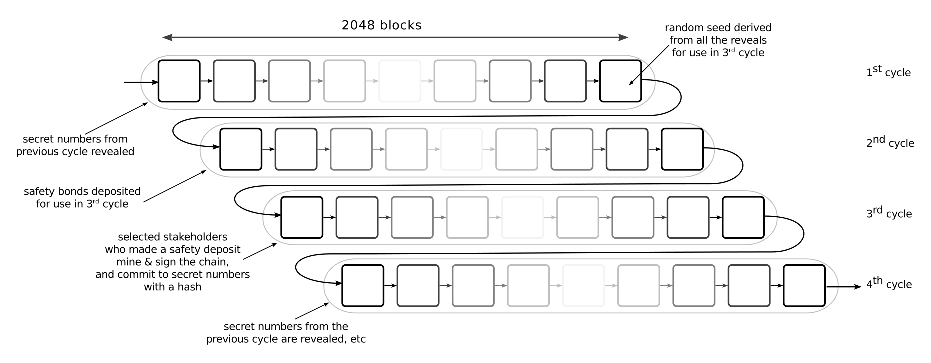
\includegraphics[width=0.8\textwidth]{pos_figure.eps}
  \caption{四阶段POS机制}
  \label{fig:pos_figure}
\end{figure}


\subsubsection{时钟}

%% The protocol imposes minimum delays between blocks. In principle, each block
%% can be mined by any stakeholder. However, for a given block, each stakeholder
%% is subject to a random minimum delay. The stakeholder receiving the highest
%% priority may mine the block one minute after the previous block. The
%% stakeholder receiving the second highest priority may mine the block two
%% minutes after the previous block, the third, three minutes, and so on.
协议在区块之间增加了最小延迟。原则上,任何一个持币人都可能挖出块。但是,就一个特定的块而言,每个持币者都将受到一个随机的最低延期的制约。
最高优先级的持币人很可能会在上一个块出现后一分钟后挖出下一个。优先级第二的持币者可能在两分钟后挖到下一个块,以此类推,优先级第三的会在三分钟后挖到下一个块。

%% This guarantees that a fork where only a small fraction of stakeholder
%% contribute will exhibit a low rate of block creation. If this weren't
%% the case, a CPU denial of service attacks would be possible by
%% tricking nodes into verifying a very long chain claimed to have a very high
%% score.
这将保证在一个分叉中持有股权较少的持币人拥有较低的出块率。否则,一个针对CPU的DDos攻击将可能欺骗节点,导致其确认一个较长的自称高得分的链。

\subsubsection{随机种子生成}

%% Every block mined carries a hash commitment to a random number chosen by the
%% miner. These numbers must be revealed in the next cycle under penalty of
%% forfeiting the safety bond. This harsh penalty is meant to prevent selective
%% whitholding of the numbers which could be sued to attack the entropy of the seed.
每一个被挖的块都会携带一个由矿工选择的随机数的哈希值。这些数字必须在下一个周期的担保金没收时间前被公开。
这个严厉的惩罚措施可以防止因矿工拒不提供随机数而有可能导致的对种子进行的熵攻击。

%% Malicious miners in the next cycle could attempt to censor such reveals, however
%% since multiple numbers may be revealed in a single block, they are very unlikely
%% to succeed.
恶意的矿工在下一个周期会试图阻止该随机数被公开,但是因为多个随机数可能会在单个区块中被公开,这样的企图很难成功。

%% All the revealed numbers in a cycle are combined in a hash list and the seed is
%% derived  from the root using the \verb!scrypt! key derivation function. The key
%% derivation should be tuned so that deriving the seed takes on the order of a
%% fraction of a percent of the average validation time for a block on a typical
%% desktop PC.
在一个周期中所有的被公开的数字都将合并到一个哈希列表中,并且这个种子将从根部通过使用\verb!scrypt!的密钥衍生函数得出。
这个密钥的衍生需要经过调试,使得衍生种子所需的时间和一台普通桌面电脑确认区块所需平均时间百分之一的一小部分的量级相当。

\subsubsection{Follow-the-coin过程}

%% In order to randomly select a stakeholder, we use a follow the coin procedure.
为了随机选取持币者,我们引入一个跟随币机制。

\paragraph{原理}
%% The idea is known in bitcoin as follow-the-satoshi. The procedures works
%% ``as-if'' every satoshi ever minted had a unique serial number. Satoshis are
%% implicitly ordered by creation time, a random satoshi is drawn and tracked
%% through the blockchain. Of course, individual cents are not tracked directly.
%% Instead, rules are applied to describe what happens when inputs are combined and
%% spent over multiple output.
这个方法最初出现在比特币中,称为follow-the-satoshi。
该过程假设每一个锻造出来的聪单位的比特币都有唯一的序列号,聪按照创建时间隐式排序,通过区块链对其操作和追踪。
当然,单个分不能够直接追踪。但是可以通过使用一些规则描述当输入集成起并通过多个输出花出时发生的情况。

%% In the end, the algorithm keeps track of a set of intervals associated with each
%% key. Each intervals represents a ``range'' of satoshis.
%% Unfortunately, over time, the database becomes more and more fragmented,
%% increasing bloat on the client side.
最后, 算法持续追踪每一组和密钥相关联的间隔。每个间隔表示聪区间的范围。不幸的是,随着时间的延长,数据库变得越来越零碎,使得客户端膨胀。

\paragraph{币卷}
%% We optimize the previous algorithm by constructing large ``coin rolls'' made up
%% of \num{10000} tez. There are thus about one million rolls in existence. A
%% database maps every roll to its current owner.
通过建立大的由一万个tez组成的币卷,我们优化之前的算法。总共会有大约一百万个卷存在。数据库把每个卷地图映射到其当前的所有者。

%% Each address holds a certain set of specific rolls as well as some loose change.
%% When we desire to spend a fraction of a full roll, the roll is broken and
%% its serial number is sent in a LIFO queue of rolls, a sort of ``limbo''. Every
%% transaction is processed in a way that minimizes the number of broken rolls.
%% Whenever an address holds enough coins to form a roll, a serial number is pulled
%% from the queue and the roll is formed again.
每一个地址都带有一个特定卷的集合,以及一些零钱。
当我们花掉只占一个卷一小部分的币时,整个卷就会被破坏,而它的序列号会发送至卷的LIFO队列,该队列有点像放置废弃物的场所。
每笔交易都应该以最小化破坏卷的方式处理。每当一个地址有足够的币来组成一个卷,序列号将从队列中拉出,再次生成卷。


%% The LIFO priority ensures that an attacker working on a secret fork cannot
%% change the coins he holds by shuffling change between accounts.
LIFO队列优先级保证了在一个秘密分叉上挖矿的攻击者无法通过账户间混洗改变的方法,达到修改其拥有的币数的目的。

%% A slight drawback of this approach is that stake is rounded down to the
%% nearest integer number of rolls. However, this provides a massive improvement
%% in efficiency over the follow-the-satoshi approach.
这样做会有一个很小的问题,那就是股份数被近似为卷值最接近的整数。但是相对于follow-the-satoshi方法,该方法在效率方面提供了很大的改善。

%% While the rolls are numbered, this approach does not preclude the use of
%% fungibility preserving protocols like Zerocash. Such protocols can use
%% the same ``limbo'' queue technique.
虽然币卷被数字化,这个方法并不能阻碍那些诸如零币那样的使用可替代性保持的协议。这些协议可以使用相同的limbo队列技术。

\paragraph{动机}
%% This procedure is functionally different from merely drawing a random address
%% weighted by balance.
上述流程和仅仅按照余额权重衡量选取随机地址的机制在功能上有很大的不同。

%% Indeed, in a secretive fork, a miner could attempt to control the generation of
%% the random seed and to assign itself signing and minting rights by creating the
%% appropriate addresses ahead of time. This is much harder to achieve if rolls
%% are randomly selected, as the secretive fork cannot fake ownership of certain
%% rolls and must thus try to preimage the hash function applied to the seed to
%% assign itself signing and minting rights.
事实上,在一个秘密的分叉内,一个矿工可以试图通过提前控制随机种子的生成和赋予自身签名和挖币的权利。
如果币卷是真正随机选择的,这种企图是很难成功,因为秘密的分叉不能够伪造某个币卷的所有权归属,
而且必须要试图来造影(preimage)在种子上应用的哈希函数,进而实现签名和造币权利的分配。

%% Indeed, in a cycle of length $N=\num{2048}$, someone holding a fraction $f$ of
%% the rolls will receive on average $f N$ mining rights, and the effective
%% fraction received, $f_0$ will have a standard deviation of
%% $$\sqrt{\frac{1}{N}}\sqrt{\frac{1-f}{f}}.$$
事实上,在一个$N=\num{2048}$周期内,某个持有币卷中一小部分$f$的人将会获得平均值为$f N$的挖矿权,
一旦接收到这个有效的部分,那么$f_0$的标准差将为:$$\sqrt{\frac{1}{N}}\sqrt{\frac{1-f}{f}}$$

%% If an attacker can perform a brute-force search through $W$ different seeds,
%% then his expected advantage is at most\footnote{this is a standard bound
%% on the expectation of the maximum of W normally distributed variable}
%% $$\left(\sqrt{\frac{2\log(W)}{N}}\sqrt{\frac{1-f}{f}}\right)fN$$
%% blocks. For instance, an attacker controlling $f = 10\%$ of the rolls should
%% expect  to mine about $205$ blocks per cycle. In a secret fork where he attempts
%% to control the seed, assuming he computed over a trillion hashes, he could
%% assign itself about $302$ blocks, or about $14.7\%$ of the blocks. Note that:
如果一个攻击者通过$W$个不同种子进行穷举式搜索,那么他的攻击的优势至多是$$\left(\sqrt{\frac{2\log(W)}{N}}\sqrt{\frac{1-f}{f}}\right)fN$$个区块。
\footnote{这是在W正态分布变量的最大期望上的标准界限。}
举个例子,一个控制了总量$f = 10\%$币卷的攻击者,他可以预期在每个周期挖大约$205$个区块。
假设他在试图控制种子的秘密分叉上有超过一万亿个哈希的算力,那么其可以分配给自己占总量区块$14.7\%$的$302$个块。值得注意的是:
\begin{itemize}
\item[-] %% The hash from which the seed is derived is an expensive key derivation
%% function, rendering brute-force search impractical.
产生种子的哈希是通过一个复杂的密钥生成函数产生的,这让穷举式搜索变得不现实。
\item[-] %% To make linear gains in blocks mined, the attacked needs to expend a
%% quadratically exponential effort.
要想在挖矿中取得线性收益,攻击者将花费平方指数级增长的资源。
\end{itemize}

\subsubsection{挖矿}
%% The random seed is used to repeatedly select a roll. The first roll selected
%% allows its stakeholder to mine a block after one minute, the second one after
%% two minutes --- and so on.
随机种子被重复用来选择币卷。第一个被选中的卷将给予它的持有者一分钟后挖块的权利,这个第二个可以在两分钟以后,以此类推。

%% When a stakeholder observes the seed and realizes he can mint a high priority
%% block in the next cycle, he can make a security deposit.
当一个持币者观察到种子并认识到他可以在下一个周期里挖掘一个高优先级的块的时候,他可以进行安全存币。

%% To avoid a potentially problematic situation were no stakeholder made a
%% safety deposit to mine a particular block, after a 16 minutes delay, the
%% block may be mined without a deposit.
存在这样一个潜在问题,即没有持有人进行安全存币购买债券来挖一个特定的块。如果这种情况发生,那么在16分钟以后,这个块就可以在没有存款的情况下被挖出。

%% Bonds are implicitely returned to their buyers immediately in any chain
%% where they do not mine the block.
当购买债券的人不在挖矿时,购买债券的币将通过隐式的方式立即返还这些购买人。

\subsubsection{区块签名}
%% As it is, we almost have a working proof of stake system.
%% We could define a chain's weight to be the number of blocks.
%% However, this would open the door to a form of selfish mining.
就这样我们构建了一个几乎完备可行的POS系统。但是一个问题是将一个链的权重定义为区块数量,这会带来自私挖矿的问题。

%% We thus introduce a signing scheme. While a block is being minted, the random
%% seed is used to randomly assign 16 signing rights to 16 rolls.
为此,我们引入了一个签名模式。当一个区块被挖出的时候,随机种子将随机分配16个签名权利给16个币卷。

%% The stakeholders who received signing rights observe the blocks being minted and
%% then submit signatures of that blocks. Those signatures are then included in
%% the next block, by miners attempting to secure their parent's inclusion in the
%% blockchain.
持币者获得签名权利后一旦观察到正在被挖出的区块就会上传区块签名。这些签名会包括在下一个区块里,该工作由试图保证区块链中父子包含关系的矿工完成。

%% The signing reward received by signers is inversely proportional to the time
%% interval between the block and its predecessor.
签名人获得的签名奖励与区块和其先祖区块之间的时间间隔成反比。

%% Signer thus have a strong incentive to sign what they genuinely believe to be
%% the best block produced at one point. They also have a strong incentive to agree
%% on which block they will sign as signing rewards are only paid if the block ends
%% up included in the blockchain.
因此,签名人有很强的意愿尽快签名他们所认为在某一时刻产生的最优的区块。他们也有很强的动机达成签名哪个区块的共识,因为签名奖励只有在区块被写入区块链后才能发放。

%% If the highest priority block isn't mined (perhaps because the miner isn't
%% on line), there could be an incentive for signers to wait for a while, just
%% in case the miner is late. However, other signers may then decide to sign the
%% best priority block, and a new block could include those signatures, leaving out
%% the holdouts. Thus, miners are unlikely to follow this strategy.
如果优先级最高的块没有被挖出(可能是因为矿工没有在线),签名人会有因为存在矿工迟到的可能性而决定等待一些时间的动机。
但是其它签名人可能会决定签名优先级最高的块,一个新块可能包含这些签名,让那些等待者一无所获,所以矿工不太可能采取等待的策略。

%% Conversely, we could imagine an equilibrium where signers panic and start
%% signing the first block they see, for fear that other signers will do so and
%% that a new block will be built immediately. This is however a very contrived
%% situation which benefits no one. There is no incentive for signers to think this
%% equilibrium is likely, let alone to modify the code of their program to act
%% this way. A malicious stakeholder attempting to disrupt the operations would only
%% hurt itself by attempting to follow this strategy, as others would be unlikely
%% to follow suit.
我们可以假设存在与之相反的情形,签名者过于担心竞争者抢先,而争相对所看到的第一个块进行签名。然而现实是这种情形其实对任何人没有什么好处。
签名者没有理由认为会出现这种状况,更不用说去修改他们的程序代码来去这样做。虽然理论上存在一个恶意的持币者试图扰乱秩序的可能,但这样只会损害自己的利益,其他人也不会效仿。

\subsubsection{链的权重}

%% The weight is the number of signatures.
我们定义链的权重为签名数。

\subsubsection{公开谴责机制}
%% In order to avoid the double minting of a block or the double signing of a
%% block, a miner may include in his block a denunciation.
为了避免一个区块上的双挖以及双签问题, 一个矿工可以在他的区块中加入一个公开谴责机制。

%% This denunciation takes the form of two signatures. Each minting signature
%% or block signature signs the height of the block, making the proof of malfeasance quite concise.
该公开谴责机制采取双签名的形式。每一个造币的签名或者块的签名都签入区块高度,构成恶意行为的证据,这让不良行为很难隐藏。

%% While we could allow anyone to denounce malfeasance, there is really no point to
%% allow anyone else beyond the block miner. Indeed, a miner can
%% simply copy any proof of malfeasance and pass it off as its own
%% discovery.\footnote{A zero-knowledge proof would allow anyone to benefit from
%% denouncing malfeasances, but it's not particularly clear this carries much
%% benefit.}
尽管我们可以允许任何人来谴责不良行为,但没有人比矿工更适合来这样做。
事实上,一个矿工可以简单地复制不良行为的证据并将其作为自己的发现转达给其他人\footnote{零知识证明允许任何人从谴责不良行为获益,但获益多少并不十分明确。}。


%% Once a party has been found guilty of double minting or double signing,
%% the safety bond is forfeited.
而一旦发现有双挖或者双签,那么其债券将被没收。

\subsection{智能合约}

\subsubsection{合约类型}
%% In lieu of unspent outputs, Tezos uses stateful accounts. When those
%% accounts specify executable code, they are known more generally as
%% contracts. Since an account is a type of contract (one with no
%% executable code), we refer to both as "contracts" in full generality.
和比特币的unspent输出不同,Tezos使用有状态的账户。当这些账户规定了可被执行的代码时,它们也就成了广泛意义上的合约。
账本本身也是一种合约,只是没有可执行的代码。

%% Each contract has a ``manager", which in the case of an account is
%% simply the owner. If the contract is flagged as spendable, the manager
%% may spend the funds associated with the contract. In addition, each
%% contract may specify the hash of a public key used to sign or
%% mine blocks in the proof-of-stake protocol. The private key may or
%% may not be controlled by the manager.
每一个合约都有一个管理者,对于账户而言,这个管理者就是它的拥有者。如果这个合约标识为可以被花费的,那也意味着管理者可以花费与这个合约相关联的资金。
此外,每一个合约都可能会规定一个公钥的哈希用来签署或者挖POS协议内的区块。私钥可由或不由管理者控制。

%% Formally, a contract is represented as:
一个合约可以正式表示为:

\begin{lstlisting}
type contract = {
  counter: int; (* counter to prevent repeat attacks *)
  manager: id; (* hash of the contract's manager public key *)
  balance: Int64.t; (* balance held *)
  signer: id option; (* id of the signer *)
  code: opcode list; (* contract code as a list of opcodes *)
  storage: data list; (* storage of the contract *)
  spendable: bool; (* may the money be spent by the manager? *)
  delegatable: bool; (* may the manager change the signing key? *)
}
\end{lstlisting}

%% The handle of a contract is the hash of its initial content. Attempting
%% to create a contract whose hash would collide with an existing contract
%% is an invalid operation and cannot be included in a valid block.
一个合约的句柄是初始内容的哈希值。试图创建的合约的哈希不能与已经存在的相同,否则将不会被包含在一个有效区块内。

%% Note that data is represented as the union type.
该数据表示为一个union类型。

\begin{lstlisting}
type data =
  | STRING of string
  | INT of int
\end{lstlisting}

%% where \verb!INT! is a signed 64-bit integer and string is an array of
%% up to \num{1024} bytes. The storage capacity is limited to \num{16384} bytes,
%% counting the integers as eight bytes and the strings as their length.
这里\verb!INT!是一个有符号的64位整数,string是一个1024字节的数组。存储空间上限为\num{16384}字节,将整数以八字节计数,strings则以它们的长度计数。

\subsubsection{起源}

%% The origination operation may be used to create a new contract, it specifies
%% the code of the contract and the initial content of the contract's storage. If
%% the handle is already the handle of an existing contract, the origination is
%% rejected (there is no reason for this to ever happen, unless by mistake or
%% malice).
起源操作可以用来创建一个新的合约,主要是合约代码和合约存储的初始内容。如果该句柄已经是一个已存在的合约的句柄,那么起源操作将被拒绝。(除非是因为错误或恶意,否则基本不会发生。)

%% A contract needs a minimum balance of $\tz~\num{1}$ to remain active. If the
%% balance falls below this number, the contract is destroyed.
合约需要最低\tz~\num{1}余额来保证其正常运行。如果这个余额低于这个数字,该合约就会被销毁。
\subsubsection{交易}

%% A transaction is a message sent from one contract to another contract, this
%% messages is represented as:
交易是从一个合约发至另一个合约的消息,可表示为:

\begin{lstlisting}
type transaction = {
  amount: amount; (* amount being sent *)
  parameters: data list; (* parameters passed to the script *)
  (* counter (invoice id) to avoid repeat attacks *)
  counter: int;
  destination: contract hash;
}
\end{lstlisting}

%% Such a transaction can be sent from a contract if signed using the manager's key
%% or can be sent programmatically by code executing in the contract. When the
%% transaction is received, the amount is added to the destination contract's
%% balance and the destination contract's code is executed. This code can make use
%% of the parameters passed to it, it can read and write the contract's storage,
%% change the signature key and post transactions to other contracts.
如果交易使用管理者密钥签名,或者以编程的方式通过合约中的程序代码执行,那么交易将从合约发出。
当这个交易被接收,该交易金额就被加入目的合约的余额中,并且执行目的合约代码。该代码可利用接收到的参数,对合约存储进行读写,改变签名密钥,以及发送交易至其它合约。

%% The role of the counter is to prevent replay attacks. A transaction is only
%% valid if the contract's counter is equal to the transaction's counter. Once a
%% transaction is applied, the counter increases by one, preventing the transaction
%% from being reused.
计数器的作用是防止中继攻击。当合约的计数等于交易的计数的时,该交易才是有效的。一旦交易被确认,计数器就会增加1,防止该交易被重用。

%% The transaction also includes the block hash of a recent block that the client
%% considers valid. If an attacker ever succeeds in forcing a long reorganization
%% with a fork, he will be unable to include such transactions, making the fork
%% obviously fake. This is a last line of defense, TAPOS is a great system to
%% prevent long reorganizations but not a very good system to prevent short term
%% double spending.
该交易也包含客户端认为有效的最近区块哈希值。如果攻击者成功地迫使一个分叉进行长重组,这些交易将不能被整合入区块链,使得分叉显得明显伪造。
这也是安全的最后一道防线,虽然TAPOS是有效防止这种长重组的伟大的系统,但是该系统对于防止短期双花并不是十分有效。

%% The pair (account\_handle, counter) is roughly the equivalent of an unspent
%% output in Bitcoin.
一个(account\_handle, counter)对和比特币中未被花掉的输出几乎等价。

\subsubsection{存储费用}

%% Since storage imposes a cost on the network, a minimum fee of \tz~1 is assessed
%% for each byte increase in the storage. For instance, if after the execution of
%% a transaction, an integer has been added to the storage and ten characters have
%% been appended to an existing string in the storage, then \tz~18 will be withdrawn
%% from the contract's balance and destroyed.
存储是网络上最重要的成本之一,在存储上每增加一个字节大约最低的费用为\tz~1。
例如,如果交易执行后,一个整数被添加到存储中,并且在已经存在的存储的字符串上增加10个字节,那么\tz~18将从合约的余额中取出和销毁。


\subsubsection{代码}

%% The language is stack based, with high level data types and primitives and strict
%% static type checking. Its design is insipired by Forth, Scheme, ML and Cat.
%% A full specification of the instruction set is available in\cite{language}.
%% This specification gives the complete instruction set, type system and semantics
%% of the language. It is meant as a precise reference manual, not an easy introduction.
该语言是基于栈的且具有高级的数据类型和严格的静态类型校验。设计的灵感来自Forth, Scheme, ML 和 Cat。它有一个完全描述的指令集\cite{language},详细描述了指令集,类型系统,以及词法和语义。
这也意味着一个精准的完全参考指南,而不是一个简单的介绍。

\subsubsection{交易费}

%% So far, this system is similar to the way Ethereum handles transaction. However,
%% we differ in the way we handle fees. Ethereum allows arbitrarily long programs
%% to execute by requiring a fee that increases linearly with the program's
%% executing time. Unfortunately, while this does provide an incentive for one
%% miner to verify the transaction, it does not provide such an incentive to other
%% miners, who must also verify this transaction. In practice, most of the
%% interesting programs that can be used for smart contracts are very short.
%% Thus, we simplify the construction by imposing a hard cap on the number of steps
%% we allow the programs to run for.
到目前为止,这个系统和以太坊处理交易的方式很类似。然而,我们在处理交易费方面却很不同。在以太坊上用户只要支付随程序执行时间线性增长的费用,就可以运行任意长的程序。
虽然这种方式提供了矿工验证交易的经济动机,但并不能给同样参与交易验证的其他矿工相同的动机。
在实践中,大多数用智能合约编写的程序都是非常短的。因此,我们通过在程序的执行步骤上加上一个硬性的帽子来简化构建过程。

%% If the hard cap proves too tight for some programs, they can break the execution
%% in multiple steps and use multiple transactions to execute fully. Since Tezos is
%% amendable, this cap can be changed in the future, or advanced primitives can be
%% introduced as new opcodes.
如果该帽子对一些程序而言被证明是紧上界,他们可以在多个执行步骤上中断并采取多个交易完全执行的方式。
正是因为Tezos是自我进化的,这个帽子在未来可以改变,或者引入更多的高级原语。

%% If the account permits, the signature key may be changed by issuing a signed
%% message requesting the change.
如果账户同意,签名密钥可以通过发起签名信息请求修改。

\section{总结}
%% We feel we've built an appealing seed protocol. However, Tezos's true potential
%% lies in putting the stakeholders in charge of deciding on a protocol that they
%% feel best serves them.
我们认为,我们已经构建一个较大吸引力的种子协议。当然,Tezos的真正的潜力存在于:让持币者掌控最优质服务协议的选择权利。

\bibliographystyle{plain}
\bibliography{biblio}

\end{document}
